%A template for assignements and examinations
%Author: Sudharshan Kaarthik R

\documentclass[11pt, a4paper, addpoints]{exam} %Exam class is used
\usepackage{lmodern} %Change font package is required lmodern for classic look, newtx for neutral look, sans for modern look
\usepackage{babel}
\usepackage{hyperref} %for resources and weblinks
\usepackage{graphicx} %for including graphics
\usepackage{microtype} %for better typesetting
\usepackage{cleveref} %for alternate usages of keywords
\usepackage{lipsum} %Only for demo, remove for normal usage
\usepackage[left=0.75in,right=0.75in,top=1in,bottom=1in,headsep=.5\baselineskip]{geometry} %Better page utilization
\pagestyle{headandfoot}
\headrule
\newcommand{\continuedmessage}{%
	\ifcontinuation{\footnotesize Question \ContinuedQuestion\ continues\ldots}{}%
}
\crefname{figure}{figure}{figures}
\crefname{question}{question}{questions}

%%%%%%%% Start editing from here %%%%%%%%

\runningheader{\footnotesize Course Code} {\footnotesize Course name} {\footnotesize Page \thepage\ of \numpages}
\footrule
\footer{\footnotesize Student's name:}{}{\ifincomplete{\footnotesize Question \IncompleteQuestion\ continues on the next page\ldots}{\iflastpage{\footnotesize End of assignment}{\footnotesize Please go on to the next page\ldots}}}



%==============================================================
\begin{document}

%=====Minipage for creating title section=====%
%=====LOGO=====Title=====Due date/exam duration====

	\noindent
	\begin{minipage}[l]{.2\textwidth}%
		\noindent
		
\includegraphics[width=0.6\textwidth]{IIST_logo}
	\end{minipage}
	\hfill
	\begin{minipage}[c]{.55\textwidth}%
		\vspace{0.1cm}
		\begin{center}
			{\bfseries Department Name \par
			   Indian Institute of Space Science and Technology \par
				\small Course Name {(\small Course Code)} \par
						Exam / Quiz / Assignment }
		\end{center}
		\vspace{0.15cm}
	\end{minipage}
	\begin{minipage}[r]{.2\textwidth}%
			\noindent
			\small
			\centering
%			Due date \\ 21 Aug, 2023 \\ %for assignments
			Exam duration: 3 hrs \\ Max. Marks: 100
	\end{minipage}
	\noindent \rule{\textwidth}{0.7pt}
%%=======================================================



% General instructions for the exam/assignemtn can be given here
	\textit{ \small Provide instructions here.}\\
	\rule{\textwidth}{0.7pt}

% Questions start here

	\begin{questions}
		\question Question 1 text to be included here.
			\begin{parts}
				\part[5] Text for part-A: \lipsum[1][1-5]
				\part[5] Text for part-B: \lipsum[2][1-5]
				\begin{subparts}
					\subpart[3] Text for Sub-part-A: \lipsum[3][1-5]
					\subpart[2] Text for Sub-part-B: A graphic can also be included.
					\begin{figure}[h]
						\centering
						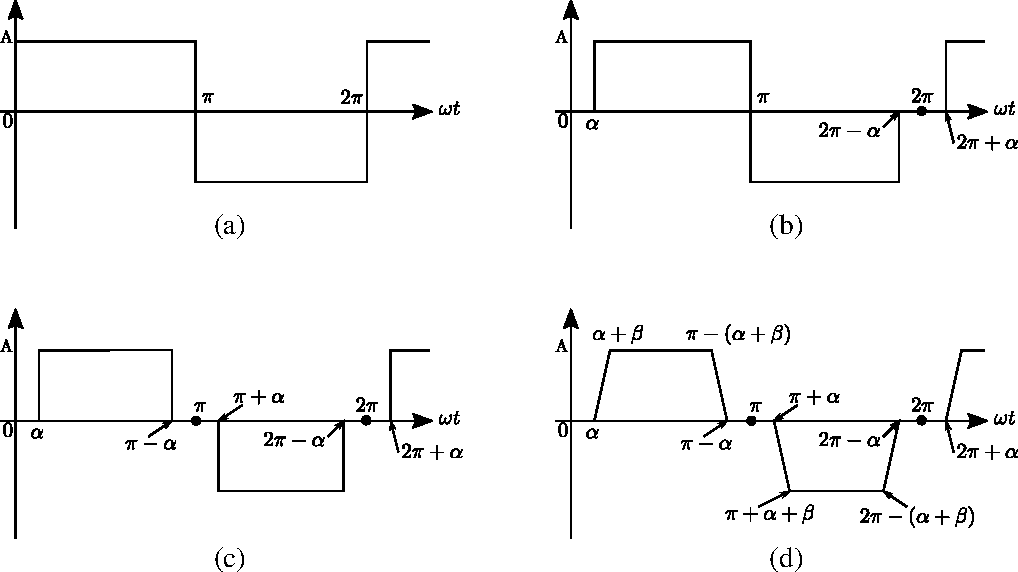
\includegraphics[width=0.7\linewidth]{Waveforms}
						\caption[Short Caption]{Figure for Q1.}
						\label{fig:waveforms}
					\end{figure}

					\begin{subsubparts}
						\subsubpart[1] Text for sub-sub-part-A: \lipsum[4][1-5]
						\subsubpart[1] Text for sub-sub-part-B: \lipsum[5][1-5]
					\end{subsubparts}
				\end{subparts}
			\end{parts}
		\droptotalpoints

		\question Question 2 text to be included here. \lipsum[6][1-5]
		\begin{parts}
			\part[5] Text for part-A: \lipsum[7][1-5]
			\part[5] Text for part-B: \lipsum[8][1-5]
			\begin{subparts}
				\subpart[3] Text for Sub-part-A.
				\subpart Text for Sub-part-B. \\
				Link can be included: \url{https://github.com/sudharshankaarthik/Inkscape_electrical_symbols.git}
			\end{subparts}
		\end{parts}

	\droptotalpoints

	\question Question 3 text to be included here. \lipsum[9][1-5]
	\question Question 4 text to be included here. \lipsum[10][1-5]
	\question Question 5 text to be included here. \lipsum[11][1-5]
	\question Question 6 text to be included here. \lipsum[12][1-5]


	Additional text can also be added: \lipsum[9][1-5]
	\begin{itemize}
		\item Additional text 1. \lipsum[10][1-3]
		\item Additional text 2. \lipsum[11][1-4]
	\end{itemize}

	\end{questions}

\noindent \rule{\textwidth}{0.7pt} %Mark end of document

\end{document}
